\documentclass[lettersize,journal]{IEEEtran}
\usepackage{amsmath,amsfonts}
\usepackage{algorithmic}
\usepackage{algorithm}
\usepackage{array}
\usepackage[caption=false,font=normalsize,labelfont=sf,textfont=sf]{subfig}
\usepackage{textcomp}
\usepackage{stfloats}
\usepackage{url}
\usepackage{verbatim}
\usepackage{graphicx}
\usepackage{lineno}
\usepackage{booktabs}
\usepackage{float}
\usepackage{xcolor}
\usepackage{tikz}
\usepackage{adjustbox}
\usepackage{pgfplots}
\usepackage{hyperref}
\usepackage[noadjust]{cite}
\newcommand*\circled[1]{\tikz[baseline=(char.base)]{
            \node[shape=circle,draw,inner sep=1pt] (char) {#1};}}

\newcommand\blfootnote[1]{%
  \begingroup
  \renewcommand\thefootnote{}\footnote{#1}%
  \addtocounter{footnote}{-1}%
  \endgroup
}
\hyphenation{op-tical net-works semi-conduc-tor IEEE-Xplore}
% updated with editorial comments 8/9/2021

\begin{document}

\title{Experience Sharing from Team National Tsing Hua University for 2023 APAC HPC-AI Competition}


\author{\IEEEauthorblockN{Zhan-Yi~Lin ~\IEEEauthorrefmark{1}, Chen-An~Pai\IEEEauthorrefmark{1}, Shih-Hsun~Wei~\IEEEauthorrefmark{1}, Hao-Tien~Yu~\IEEEauthorrefmark{1}, Shih-Jou~Cheng~\IEEEauthorrefmark{1}, Chih-Yu~Hsieh~\IEEEauthorrefmark{1}, Tung Yu~Hsieh ~\IEEEauthorrefmark{1}, Wei-Chih~Huang~\IEEEauthorrefmark{1}, Ssu-Cheng~Lai~\IEEEauthorrefmark{1}, Wei-Po~ Lin~\IEEEauthorrefmark{1}, Chan-Yu~Mou~\IEEEauthorrefmark{2}, Jerry Chou~\IEEEauthorrefmark{2},}
\IEEEauthorblockA{Department of Computer Science, National Tsing Hua Univeristy, Taiwan \\ \IEEEauthorrefmark{1} contributed equally to this work as first authors \\ \IEEEauthorrefmark{2} corresponding author}
}

% The paper headers
\markboth{SupercomputingAsia 2024}%
{Huang and Chang \MakeLowercase{\textit{et al.}}: A Sample Article Using IEEEtran.cls for IEEE Journals}

% \IEEEpubid{0000--0000/00\$00.00~\copyright~2021 IEEE}
% Remember, if you use this you must call \IEEEpubidadjcol in the second
% column for its text to clear the IEEEpubid mark.

\maketitle

\blfootnote{Jerry Chou is the corresponding author and team advisor who guided the team to compete this study and writing. All authors approve of the content of the manuscript and agree to be held accountable for the work.}



\begin{abstract}
As part of the Student Cluster Competition at the SC22 conference, this work aims to reproduce the performance evaluations of the Data Centric (DaCe) Python framework by leveraging Intel MKL and NVIDIA CUDA interface. The evaluations are conducted on a single CPU-based node, NVIDIA A100 GPUs, and a eight-node cloud supercomputer. Our experimental results successfully reproduce the performance evaluations on our cluster. Additionally, we provide insightful analysis and propose effective methods for achieving higher performance when utilizing DaCe as an acceleration library.
\end{abstract}


\begin{IEEEkeywords}
Student Competition, Performance Optimization, AI\end{IEEEkeywords}

\section{Introduction}
\label{sec:intro}
%\IEEEPARstart{A}{s} a special activity of the Student Cluster Competition at SC22 conference, we made an attempt to reproduce the performance evaluations of the \textit{Data-Centric (DaCe) Python framework} \cite{dace2021}. Ihis work aims to reproduce the results reported in \cite{dace2021} on a 4-node cluster equipped with AMD Zen 3 processors \cite{amdCPU} and NVIDIA A100 \cite{nvA100}.
% \IEEEPARstart{M}any frameworks are been proposed to support high-performance computing (HPC) with Python. For instance, Numba \cite{lam2015numba} is a just-in-time (JIT) compiler which translates a portion of Python code to pre-compiled machine code; NumPy features utilizing SIMD instructions and BLAS libraries. In addition, MPI4PY \cite{mpi4py} makes writing Python code with message passing interface (MPI) possible to support distributed computing. 


% \IEEEPARstart{P}ython has become one of the most used language \cite{dace2021}. Benefited from
% the NumPy \cite{harris2020array} library, many frameworks based on NumPy has developed, such as SciPY, Matplotlib, scikit and pandas. These frameworks make writing Python code with ease, and therefore are highly employed by both developers and users for scientific simulation \cite{2016md_simulation, ziogas2019quantum} and machine learning\cite{tensorflow2015-whitepaper,2019pytorch} domains.  As a result, several optimization libraries have been proposed to support high-performance computing (HPC) with Python. For instance, Numba \cite{lam2015numba} is a just-in-time (JIT) compiler which translates a portion of Python code to pre-compiled machine code; NumPy \cite{harris2020array} features utilizing SIMD instructions and BLAS libraries. In addition, MPI4PY \cite{mpi4py} makes writing Python code with message passing interface (MPI) possible to support distributed computing. 
\IEEEPARstart{P}ython has become one of the most widely used languages~\cite{dace2021} for scientific code. Its popularity is attributed to the availability of numerous frameworks based on NumPy~\cite{harris2020array}, such as SciPy~\cite{2020SciPy-NMeth}, scikit-learn~\cite{scikit-learn}, and pandas~\cite{mckinney-proc-scipy-2010}, which make writing Python code easier. These frameworks are extensively employed by developers and users in scientific simulation~\cite{2016md_simulation, ziogas2019quantum} and machine learning~\cite{tensorflow2015-whitepaper,2019pytorch} domains. However, existing Python libraries for high-performance computing (HPC) lack simultaneous support for the three Ps~\cite{20203P,dace2021}: Productivity, Portability, and Performance.
 
% Nonetheless, none of the existing libraries supports the three Ps \cite{20203P} (Productivity, Portability, Performance) on Python at the same time. Therefore, the Data-Centric (DaCe) Python \cite{dace2021} is proposed to bridge the gap. First, by using some annotating statements, users could easily employ DaCe to the existing program (Productivity). Second, DaCe provides several computing backend compatibilities such as CPU, GPU, FPGA and distributed computing (Portability). Last, DaCe could provide significant performance improvement compared the state-of-the-art libraries (Performance).
To bridge this gap, the Data-Centric (DaCe) Python framework~\cite{dace2021} is proposed. DaCe offers several advantages. Firstly, it allows users to integrate it into existing programs using annotating statements, enhancing productivity. Secondly, DaCe provides compatibility with various computing backends, including CPUs, GPUs, FPGAs, and distributed computing, ensuring portability. Lastly, DaCe demonstrates significant performance improvements compared to state-of-the-art libraries. DaCe identifies data parallelism and data reusing patterns in dataflows, optimizing them and converting Python functions to C code. The resulting code can be compiled to run efficiently on CPUs, GPUs, or FPGAs.

In this work, as part of the Student Cluster Competition (SCC) at the SC22 conference, we aim to reproduce the performance evaluations of DaCe on CPUs, GPUs, and multi-node supercomputers. Our cluster includes state-of-the-art CPUs and GPUs. Despite running on different architectures (Intel Xeon 6130 CPU and NVIDIA V100 GPU in \cite{dace2021}), our results successfully reproduce the evaluation work presented by the authors~\cite{dace2021}. The contributions of this paper are as follows: 
\circled{1}~We reproduced the CPU experiments on NumPy and DaCe.
\circled{2}~We reproduced the DaCe GPU experiments against NumPy.
\circled{3}~We reproduced the distributed experiments with the scale of at most eight nodes.
\circled{4}~We provide a comprehensive analysis of the benchmarks to explain how DaCe achieves performance enhancements.

The remainder of the paper is organized as follows: Section~\ref{sec:exp-setup} presents the hardware and software configurations used in the experiments. Section~\ref{sec:exp-run} describes the experimental procedures. Sections~\ref{sec:cpu-result}, \ref{sec:gpu-result}, and \ref{sec:distributed-result} evaluate the experiments. Finally, Section~\ref{sec:conc} concludes the paper.
\section{Experimental Setup}
\label{sec:exp-setup}

\subsection{Hardware configuration}
Our testing environment comprises the GADI system at the National Computational Infrastructure(NCI) in Singapore, the ASPIRE 2A system  at  the National Supercomputing Centre (NSCC) in Singapore and the Taiwania 3 system at the National Center for High-performance Computing (NCHC) in Taiwan . In the context of the MPAS-Atmosphere application, we utilized the normal queue on GADI and Taiwania 3. Additionally, on the other hand, for Bloom application, we employed the gpuvolta queue on GADI and Taiwania 2, while opting for the normal queue on the ASPIRE 2A system.

\begin{table*}[t]
    \centering
    \caption{The cluster hardware configuration}
    \begin{tabular}{l|llll}
        \toprule
        Type & GADI & Taiwania 3  & Taiwania 2 & ASPIRE 2A\\
        \midrule
        CPU model & Intel Xeon Platinum 8274 & Intel Xeon Platinum 8280 & Intel Xeon Gold 6154 & CPU AMD EPYC 7713\\
        CPU micro architecture & Cascade Lake & Cascade Lake & Skylake & Millan \\
        CPU frequency & 3.2 GHz & 2.4 GHz & 3.0 GHz & 2 GHz\\
        Cores per CPU & 24 & 28 & 18 & 32\\
        Numbers of CPU per node & 2 & 2 & 2 & 2\\
        RAM per node & 192GB & 192GB & 192GB &  512 GB   \\
        GPUs per node &  4 $\times$ NVIDIA V100 & Not Available & 8 $\times$ NVIDIA V100 & 4 $\times$ NVIDIA A100 \\
        Infiniband    & 200 Gb/s & 100 Gb/s & 100 Gb/s  \\
        \bottomrule
    \end{tabular}
    \label{table:hardware}
\end{table*}

Table~\ref{table:hardware} summarizes some detailed hardware configurations. Our final result for MPAS-A consists of 32 CPU nodes with 48 CPU cores on each nodes, for Bloom inference, we utilized a total of 8 V100 GPUs distributed across two nodes on both GADI and Taiwania 2. Additionally,8 A100 GPUs were employed on two nodes on NSCC. . 


\subsection{Software Configuration}
Table~\ref{table:software-CPU} lists the software installed on both the GADI and Taiwania 3 cluster, which is mainly used for MPAS-A application, moreover, we have Rocky Linux as operating system on GADI and CentOS on Taiwania 3.

\begin{table}[ht]
    \centering
    \caption{The cluster software configuration for MPAS-A}
    \begin{tabular}{ll}
        \toprule
        Libraries & Versions  \\
        \midrule
        C Compiler & ICC 2021.10.0 \\
        MPI Library & OpenMPI 4.1.5 \\
        HDF5 & 1.8.18 \\
        PNETCDF & 1.12.3 \\
        NETCDF C & 4.8.1 \\
        NETCDF Fortran & 4.6.1 \\
        Parallel I/O & 2.5.10 \\
        Metis & 5.1.0 \\
        \bottomrule
    \end{tabular}
    \label{table:software-CPU}
\end{table}

Table~\ref{table:software-GPU} lists the software required from Bloom and installed on both the GADI ,Aspire2A and Taiwania 2 cluster. Furthermore, ASPIRE 2A use Red Hat Enterprise Linux 8 (RHEL) as operating system and Taiwania 2 use CentOS as operating system.

\begin{table}[ht]
    \centering
    \caption{The cluster software configuration for Bloom}
    \begin{tabular}{ll}
        \toprule
        Libraries & Versions  \\
        \midrule
        C Compiler & GCC 10.3.0 \\
        GPU Compiler & CUDA nvcc 11.6 \\
        python & 3.8 \\
        NCCL & 2.18 \\
        Pytorch & 1.12.1 \\
        Transformer & 4.26.1 \\
        Deepspeed & 0.7.6 \\
        accelerate & 0.16.0  \\
        gunicorn & 20.1.0 \\
        uvicorn & 0.19.0 \\
        jinja2 & 3.1.2 \\
        pydantic & 1.10.2 \\
        huggingface hub & 0.12.1 \\
        grpcio-tools & 1.50.0 \\
        bitsandbytes & 0.41.1 \\

        \bottomrule
    \end{tabular}
    \label{table:software-GPU}
\end{table}
\section{Description Of Applications}
\label{sec:conc}

We briefly explained some limitation and introduction of the tasks here. MPAS-Atmosphere is limited to use CPU to run the application, and the Bloom inference tasks is limited to run by GPU, moreover, MPAS-Atmosphere has to be ran on 32 nodes with 48 CPU core per node, and the Bloom inference should be done on 2 nodes with 4 GPU per node.

\subsection{MPAS-Atmosphere}
MPAS-Atmosphere is a climate model designed to simulate and study the behavior of the Earth's atmosphere, and it is based on unstructured centroidal Voronoi (hexagonal) meshes using C-grid staggering and selective grid refinement. This unstructured voronoi grid is good for scaling on parallel computers. The task is to run the 10km benchmark provided from MPAS with config dt (per step size) set to 60 and config run duration set to 16 minutes.

\subsection{Bloom}
BLOOM, a multilingual language model with 176 billion parameters, making it one of the world's largest open multilingual language model. It has the capability to generate text in 46 natural languages and 13 programming languages.The task is to run an int8 model type with deepspeed inference scripts to optimize throughput performance,aiming for the lowest throughput per token, including tokenization time (measured in milliseconds).
\pgfplotsset{compat=1.17}

\section{MPAS-Atmosphere Result}
\label{sec:conc}

\subsection{C and MPI Compiler selection}
For our first approach, we've tested out different C and MPI compiler combination. The result shows ICC 2021.10.0 with OpenMPI 4.1.5 is the best suite for MPAS, which outperformed other combination when running MPAS on the 32 nodes. 

\begin{figure}[ht]
  \centering
  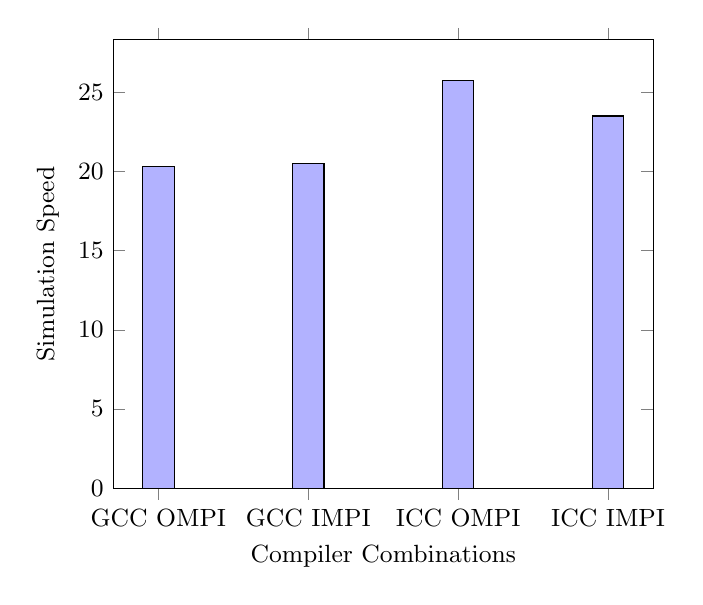
\begin{tikzpicture}
    \begin{axis}[
      ybar,
      bar width=0.4cm,
      xlabel={Compiler Combinations},
      ylabel={Simulation Speed},
      symbolic x coords={GCC OMPI, GCC IMPI, ICC OMPI, ICC IMPI},
      xtick=data,
      ymin=0,
      xticklabel style={font=\small},
      yticklabel style={font=\small},
      xlabel style={font=\small},
      ylabel style={font=\small},
    ]
      \addplot[fill=blue!30] coordinates {(GCC OMPI, 20.34) (GCC IMPI, 20.48) (ICC OMPI, 25.7474) (ICC IMPI, 23.5069)};
    \end{axis}
  \end{tikzpicture}
  \caption{ICC 2021.10.0 with OpenMPI 4.1.5 outperforms GCC with OpenMPI, GCC with IntelMPI and ICC 2021.10.0 with IntelMPI on the 32 nodes MPAS testcase.}
  \label{fig:bar_chart}
\end{figure}

\subsection{CPU Affinity}
With two CPUs on each node, we have to make sure the process binding is consisted during runtime, and the socket they are placing is correct. At the end, we chose to bind the core to hwthread and place them in the correct socket by --bind-to and --map-by from mpirun command line option. On the 32 nodes MPAS testcase, the average time is 0.3\% faster with process binding than without.

\subsection{Compile Time Flag}
We invoke the \texttt{-march}, \texttt{-ax}, and \texttt{-Ofast} flag in compiling. Since we know the architecture of the machine so setting the corresponding \texttt{-march} flag should have a significant performance increase. As the result, the first two flags really works well on MPAS, especially when \texttt{-march} flag is set to \texttt{core-avx2}. It shows the overall integration time is reduced by 4 seconds, which is almost a 10\% performance improvement. For the \texttt{-Ofast} flag, it didn't corrupt the result while it barely get any performance improvement.


\subsection{Link Time Flag}
As we are using Intel ICC compiler, we should always try the \texttt{-ipo} flag which enables multi-file interprocedural optimization in linking phase. Although we barely get any performance improvements after we tried, but theoretically, it should work well with a large application like MPAS.

\subsection{Parallel IO variables in MPAS}

In the running file of MPAS, a file called \texttt{namelist.atmosphere} stores the parameters used in simulation. There are two variables related to Parallel IO library is \texttt{config\_pio\_num\_tasks} and \texttt{config\_pio\_strides}. The fundamental rules to tune these two variables is to keep the product of them equals to the number of MPI tasks we used, which is

\begin{align*}
     config\_pio\_num\_tasks \times config\_pio\_strides\\
    = Total\;MPI\;tasks
\end{align*}

We tune these two parameters based on this equation, and tried with three different configurations, which are (32, 48), (48, 32), and (64, 24) for \texttt{config\_pio\_num\_tasks} and \texttt{config\_pio\_strides} respectively for 32 nodes (total 1536 MPI tasks). The result is shown in Fig.~\ref{fig:config-pio}.

\begin{figure}[htb]
    \centering
    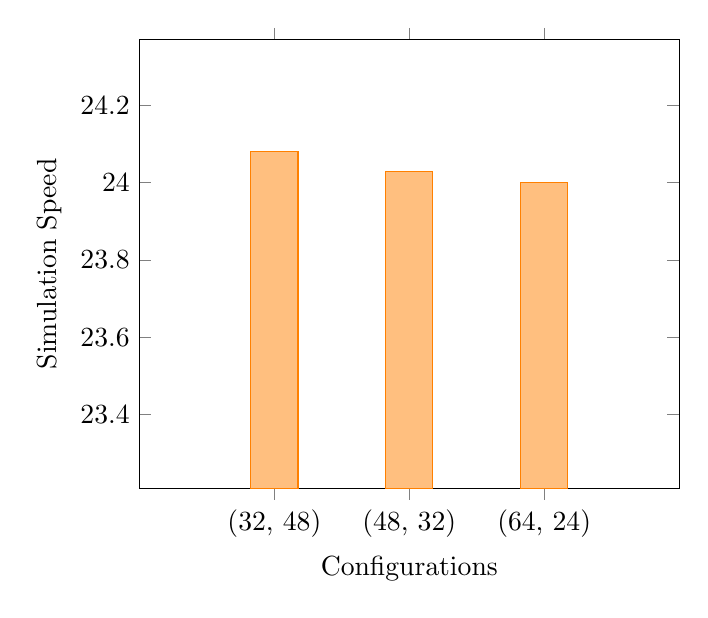
\begin{tikzpicture}
        \begin{axis}[
            ybar,
            bar width=0.6cm,
            xlabel={Configurations},
            ylabel={Simulation Speed},
            ymin=23.5,
            symbolic x coords={\text{(32, 48)}, \text{(48, 32)}, \text{(64, 24)}},
            xtick=data,
            enlargelimits=0.5,
        ]
        \addplot[
            color=orange,
            fill=orange,
            fill opacity=0.5
        ] coordinates {(\text{(32, 48)}, 24.08) (\text{(48, 32)}, 24.03) (\text{(64, 24)}, 24)};
        \end{axis}
    \end{tikzpicture}
    \caption{Simulation Speed with different PIO parameters in MPAS. All of them uses 32 nodes to get the best performance.}
    \label{fig:config-pio}
\end{figure}

We can see that when the configurations on these two parameters matches the nodes we used and the hardware threads on each machine, MPAS performances slightly better cause they matches the number of nodes and hardware threads performing I/O operations. We've gained about 0.3\% of performance increase from here.

\subsection{Graph Load-Balancing}
After all these basic compiler and related flag settings, we start to analyze the IPM profiling result. In Fig.~\ref{figure:profile-before} we found that the load-balancing didn't seem really well on MPAS. We guess it was caused by the way MPAS partitioning the mesh and it should be able to resolve by giving different Metis setup. 

\begin{figure}[h]
    \centering
    \includegraphics[width=0.5\textwidth]{profileBefore.JPG} 
    \caption{Load balancing of MPI functions according to simulation time (without I/O)}
    \label{figure:profile-before}
\end{figure}

After some research, we found that we were able to change the load balancing tolerance in Metis. Also, another important option is selecting \texttt{objtype} (the mesh optimize mode) from optimization for edge cuts to optimization for communication. After several tests, we discovered that the latter option always have a bit higher simulation speed.

\begin{table}[ht]
    \centering
    \caption{Metis Configuration Comparison}
    \begin{tabular}{lll}
        \toprule
        Type & Default & Optimize  \\
        \midrule
        Objtype & Edge Cuts (cut) & Communication (vol) \\
        Edge cuts & 350158 & 347823 \\
        Communication volume & 354760 & 352425 \\
        Balance & 1.015 & 1.004 \\
        \bottomrule
    \end{tabular}
    \label{table:metis-configuration}
\end{table}

Then, we profile again after our work. The balancing issue has improved a little bit since the peak in the graph has dropped from 1.6 to 1.4 in Fig.~\ref{figure:profile-after}. In conclusion, we got only 1\% faster in simulation time, but we believe it may impact more in some longer or larger testcases.

\begin{figure}[h]
    \centering
    \includegraphics[width=0.5\textwidth]{profile.JPG} 
    \caption{Load balancing of MPI functions according to simulation time (without I/O) after our approach}
    \label{figure:profile-after}
\end{figure}

\subsection{I/O optimization}
Due to the longer integration step occurring every simulated 10 minutes, we suspect that there may have I/O operations causing delays. Thus, we've tried different I/O optimization attempts to solve this issue. A simple attempt is set some ROMIO environment variables to boost up the I/O. By setting romio\_cb\_read or romio\_cb\_write, which can enable, disable or let the program select the activation of the collecting buffering. In our best approach, we enable both of them. This easy setup has saved a lot of time on waiting I/O events.

\subsection{OpenMPI and UCX Configuration}
One of the best way to have better performance is to have better communication tools. UCX and MPI configuration may be the most important part in CPU task. In UCX, we turn off all the debugging flags and also turn off the verbs support since it have worse performance than other methods in OpenMPI 4.1.5. Moreover, we enable the ud, rc support and the knem support. For OpenMPI 4.1.5, we also turn off all the debugging flags and disable the verbs support. In addition, we use the hcoll and romio to support optimized communication operations, and enables the lustre support for MPI and lustre $+$ ufs for ROMIO filesystem type. Last but not least, we enable the sparse group support and use the \texttt{mellanox/optimized} option by setting \texttt{--with-platform} flag.

\subsection{Final results on Gadi and Taiwania3}
After all the approaches were done, the best results with 8, 16, 32 nodes from two different setup on Gadi and Taiwania 3 are shown in Fig.~\ref{figure:final-result}.

\begin{figure}[h]
\centering
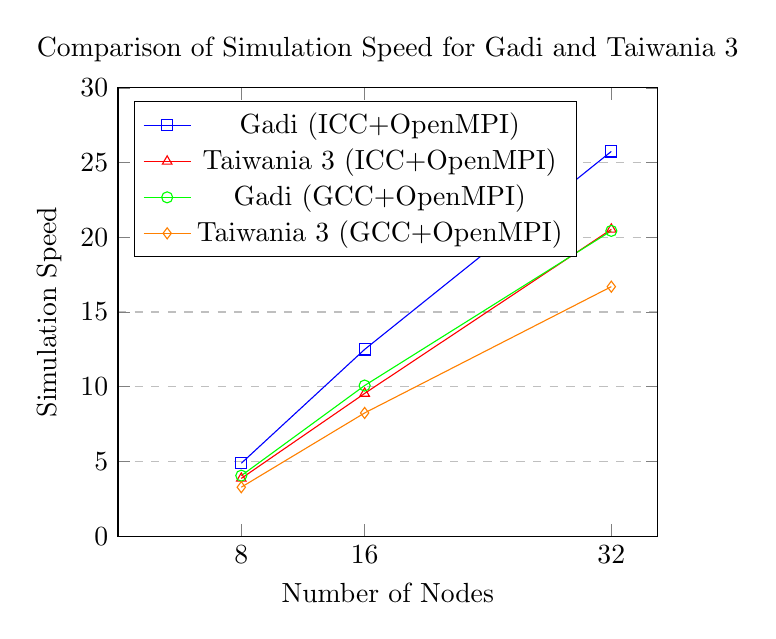
\begin{tikzpicture}
\begin{axis}[
    title={Comparison of Simulation Speed for Gadi and Taiwania 3},
    xlabel={Number of Nodes},
    ylabel={Simulation Speed},
    xmin=0, xmax=35,
    ymin=0, ymax=30,
    xtick={8, 16, 32},
    ytick={0, 5, 10, 15, 20, 25, 30},
    legend pos=north west,
    ymajorgrids=true,
    grid style=dashed,
]

% ICC + OpenMPI
\addplot[
    color=blue,
    mark=square,
    ]
    coordinates {
    (8, 4.8811)(16, 12.4976)(32, 25.7474)
    };
    \addlegendentry{Gadi (ICC+OpenMPI)}

\addplot[
    color=red,
    mark=triangle,
    ]
    coordinates {
    (8, 3.8668)(16, 9.5514)(32, 20.5316)
    };
    \addlegendentry{Taiwania 3 (ICC+OpenMPI)}

% GCC + OpenMPI
\addplot[
    color=green,
    mark=o,
    ]
    coordinates {
    (8, 4.0511)(16, 10.081)(32, 20.43)
    };
    \addlegendentry{Gadi (GCC+OpenMPI)}

\addplot[
    color=orange,
    mark=diamond,
    ]
    coordinates {
    (8, 3.2786)(16, 8.2471)(32, 16.6974)
    };
    \addlegendentry{Taiwania 3 (GCC+OpenMPI)}

\end{axis}
\end{tikzpicture}
\caption{Comparison of simulation speed between Gadi and Taiwania 3 with ICC and GCC compilers and OpenMPI on testcases with different nodes.}
\label{figure:final-result}
\end{figure}

\pgfplotsset{compat=1.17}

\section{Bloom Result}
\label{sec:conc}
In the competition, we are asked to minimize the benchmarking parameter "Throughput per token including tokenize" as much as we can. To simplify the meaning of this parameter, we can describe it as : \\
\[\Phi_{token} = \frac{t_{gen} + t_{tokenize}}{n_{gen}}\]

Since the \(t_{tokenize}\) is far smaller than \(t_{gen}\), we can rewrite the equation as : \\
\[\Phi_{token} = \frac{t_{gen}}{n_{gen}}\]

In this formula, \(t_{gen}\) represents the generation time required, \(t_{tokenize}\) represents the tokenizing time required and \(n_{gen}\) is the number of new token generated. To reduce the overall throughput per token of the BLOOM inference process, we can either increase the token inlet such that more token are generated, decrease the execution time, or both.

\subsection{Batch size}
Our first strategy is increasing the total token inlet. By using Pytorch Deep Learning framework, we can easily transfer data from host to devices in pursue of better parallel ability.

Table IV lists all sentences that will be fed as the input tokens.We found that the sentences will be duplicated several times in the list until the content in the list exceeds the batch\_size. Then, we will extract the first batch\_size sentences and feed them into the language model.

\begin{table}[ht]
    \centering
    \caption{The input sentences for BLOOM inference}
    \begin{tabular}{ll}
        \toprule
        Input\_sentences  \\
        \midrule
        "DeepSpeed is a machine learning framework" \\
        "He is working on" \\
        "He got all" \\
        "Everyone is happy and I can" \\
        "The new movie that got Oscar this year" \\
        "In the far far distance from our galaxy," \\
        "Peace is the only way" \\
        \bottomrule
    \end{tabular}
    \label{table:software-GPU}
\end{table}

By experiments, we have found that the benchmarking parameter decrease as we increasing the batch\_size.

\begin{figure}
\centering
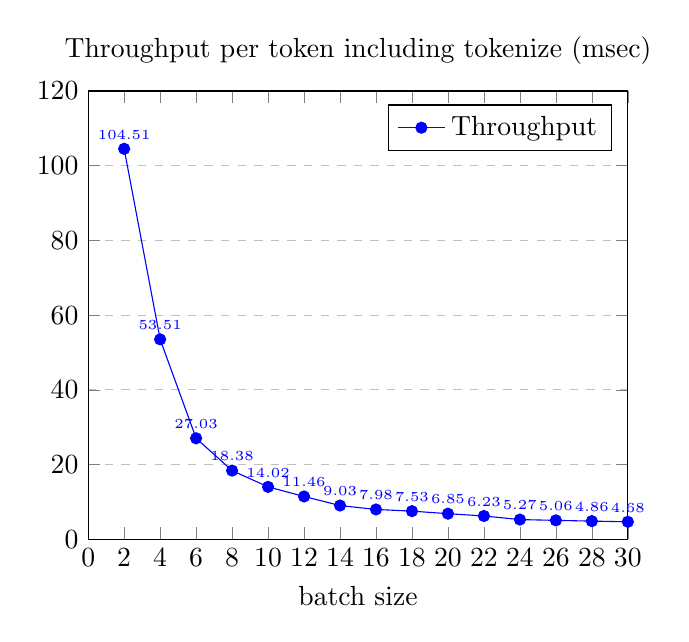
\begin{tikzpicture}
\begin{axis}[
    title={Throughput per token including tokenize (msec)},
    xlabel={batch size},
    ylabel={},
    xmin=0, xmax=30,
    ymin=0, ymax=120,
    xtick={0,2,...,30},
    ytick={0,20,40,60,80,100,120},
    legend pos=north east,
    ymajorgrids=true,
    grid style=dashed,
    every node near coord/.append style={font=\tiny},
]

\addplot[
    color=blue,
    mark=*,
    nodes near coords,
    point meta=explicit symbolic, % Allows individual points to be labeled
    ]
    coordinates {
    (2,104.51) [104.51]
    (4,53.51) [53.51]
    (6,27.03) [27.03]
    (8,18.38) [18.38]
    (10,14.02) [14.02]
    (12,11.46) [11.46]
    (14,9.03) [9.03]
    (16,7.98) [7.98]
    (18,7.53) [7.53]
    (20,6.85) [6.85]
    (22,6.23) [6.23]
    (24,5.27) [5.27]
    (26,5.06) [5.06]
    (28,4.86) [4.86]
    (30,4.68) [4.68]
    };
    \legend{Throughput}

\end{axis}
\end{tikzpicture}
\caption{Throughput per token including tokenize to batch size in two ASPIRE-2A A100x4 nodes}
\end{figure}


\subsection{Deepspeed Optimization}
Here comes another strategy. The framework we choose for Bloom is Deepspeed. It is an open-source deep learning optimization library developed by Microsoft. It is designed to enhance the training efficiency and scalability of large deep learning models. 
Deepspeed adopts three optimizations:
\subsubsection{Tensor parallelism}
In contrast, Tensor Parallelism involves the division of tensors across multiple GPUs, with each GPU handling a portion of the computation. This means that all GPUs are actively engaged in the processing simultaneously. Upon completing their respective computations, the GPUs exchange results through communication, allowing them to proceed to the next layer. By this approach, all GPUs can work simultaneously, resulting in a better overall performance.

\subsubsection{Custom CUDA Kernels}
DeepSpeed inference leverages custom CUDA kernels to minimize excessive memory allocation and inter-GPU tensor copying. As a result, this approach reduces memory requirements and decreases kernel startup overhead, leading to improved throughput and the ability to work with larger batch sizes, ultimately resulting in higher overall throughput.

\subsubsection{Mixture of Quantization}
Mixture of Quantization involves loading INT8 data from memory and converting it to FP16 before utilizing it in inference computations. This approach leverages the BitsAndBytes Python package to achieve these conversions. The key advantages include model size reduction and a substantial decrease in the inference cost during production.

\subsection{NCCL Optimization}
Here are some NCCL environment variables that we have found useful.
\subsubsection{NCCL\_NET\_GDR\_READ}
We set this variable to 1 (default 0 in non-NVlink based platform) to use GPU Direct RDMA to send data to the NIC directly.
\subsubsection{NCCL\_IB\_QPR\_PER\_CONNECTION}
We set this variable to "SYS" to always enable GPU Direct RDMA even across NUMA nodes.
\subsubsection{NCCL\_NTHREADS}
By default, V100 on Gadi use 256 threads only. We set this variable to 512 to enlarge the CUDA threads per CUDA blocks. Increasing this variable can increase the GPU clock rate.
\subsubsection{NCCL\_BUFFSIZE}
This variable control the size of buffer used by NCCL when communicating between pairs of GPUs. By experiment, we have found that setting buffer size to 8Mb gives the best performance on Gadi.



\subsection{Comparison between Gadi and Taiwania2}

\begin{figure}[h!]
\centering
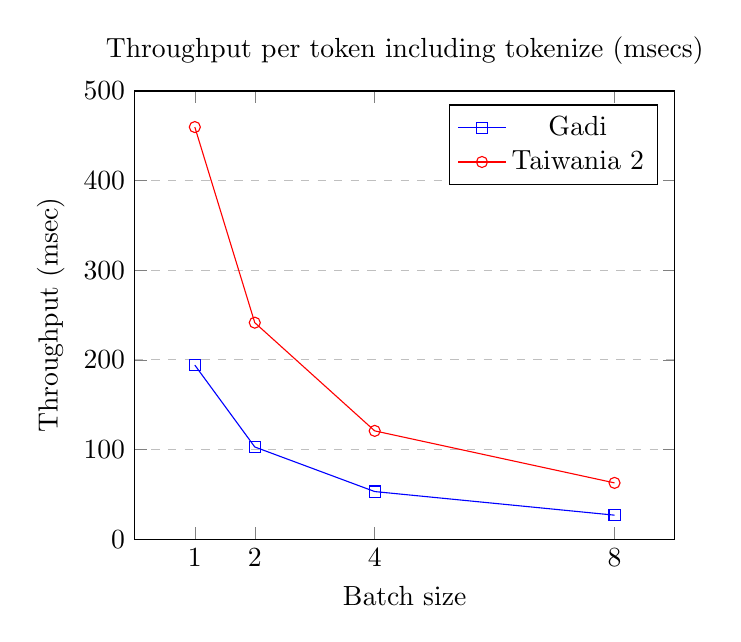
\begin{tikzpicture}
\begin{axis}[
    title={Throughput per token including tokenize (msecs)},
    xlabel={Batch size},
    ylabel={Throughput (msec)},
    xmin=0, xmax=9,
    ymin=0, ymax=500,
    xtick={1,2,4,8},
    ytick={0,100,200,300,400,500},
    legend pos=north east,
    ymajorgrids=true,
    grid style=dashed,
]

% Gadi data
\addplot[
    color=blue,
    mark=square,
    ]
    coordinates {
    (1,194.23)(2,102.93)(4,53.2)(8,26.87)
    };
    \addlegendentry{Gadi}

% Taiwania 2 data
\addplot[
    color=red,
    mark=o,
    ]
    coordinates {
    (1,459.72)(2,241.56)(4,120.88)(8,62.87)
    };
    \addlegendentry{Taiwania 2}

\end{axis}
\end{tikzpicture}
\caption{Comparison of throughput for Gadi and Taiwania 2 across different batch sizes.}
\end{figure}


\subsection{Unsuccessful Attempts}
We've also tried to use some optimization tools provided by NVIDIA, but failed to achieve any significant improvement in our results.
\subsubsection{FasterTransformer}
We've tried FasterTransformer since it claims that it provides some optimizations such as layer fusion, caching, support of multi-node, matmul kernel auto-tunning, etc.
However, it didn't have directly support of our BLOOM-176B model. Therefore we turned to other tools after successfully building the required image.
\subsubsection{TensorRT}
We've also tried TensorRT, which we thought can make use of the TensortRT inference engine to improve the performance.
It first requires to convert BLOOM to ONNX format. Unfortunately, BLOOM-176B is such a large model that it's lots of work for us to transform the entire model. We make a pause after converting the first layer of BLOOM-176B.
\subsubsection{TensorRTLLM}
Our last attempt was TensorRTLLM, which was just released recently. We thought it was the most suitable tool for us to use as its name showed. Not only it incorporates the desirable optimizations, such as kernel fusion, Tensor engine, ... some formally provided by FasterTransformer and TensorRT, it also provides python API and direct support of BLOOM-176B.
Thought finding such powerful tool, we still fail to build TensorRT engine due to memory issue, as we encountered when using TensorRT.

To sum up, almost all the attempts failed due to insufficient memory, which is unsolvable. Therefore, although they provide many desirable optimizations, these tools are not feasible in our cases.
\section{Conclusion}
\label{sec:conc}
In this work, our reproducibility experiments on a single CPU node, a single GPU, and a multi-node distributed setup confirm the effectiveness of DaCe in enhancing application performance. 
We observed consistent improvements compared to the numpy library across various benchmarks. Additionally, we provided valuable insights into optimizing DaCe's performance.

By analyzing the experiments, we discovered important factors that impact DaCe's performance. Firstly, we found that excessive use of OpenMP threads for atomic operations in CPU benchmarks can lead to significant performance degradation. By determining the optimal number of OpenMP threads, we were able to mitigate this issue and improve overall performance. Secondly, we emphasized the critical role of identifying data dependencies. By annotating critical loops, we observed substantial speedup in certain benchmarks. Finally, in GPU computations, we highlighted the potential bottleneck of communication and synchronization between the CPU and GPU, especially in cases where benchmarks are not highly parallel or involve numerous scalar operations.

It is worth noting that the artifacts provided in \cite{dace2021} make it possible for others to conduct experiments on different architectures. However, one ongoing challenge in employing DaCe is deploying applications onto GPUs, as some benchmarks couldn't be successfully executed on the GPU. Further development to fully support GPUs would advance the maturity of the DaCe framework as an HPC library.

Overall, our reproducibility efforts not only validated the findings of the original work but also provided additional insights for optimizing DaCe's performance. These findings are valuable for researchers and practitioners seeking to leverage DaCe for high-performance computing, enabling them to make informed decisions and achieve better performance in their applications. 

\bibliographystyle{IEEEtran}
\bibliography{refs.bib}

% \begin{IEEEbiography}[{\includegraphics[width=1in,height=1.25in,clip,keepaspectratio]{johnson.jpg}}]{Wei-Fang Sun}
% is pursuing his B.S. degree in Computer Science at National Tsing Hua University (NTHU). Mr. Sun's current research interests include high-performance computing, deep reinforcement learning (DRL), and robotics. His recent works focus on multi-agent reinforcement learning algorithms and DRL applications on robots.
% \end{IEEEbiography}

% \vspace{-4em}
% \begin{IEEEbiography}[{\includegraphics[width=1in,height=1.25in,clip,keepaspectratio]{imgs/bib/jchou.jpg}}]{Jerry Chou}
% received Ph.D. degree from the Department of Computer Science and Engineering at University of San Diego (UCSD) in 2009. Dr. Chou joined the Department of Computer Science at National Tsing Hua University in 2011 as an Assistant Professor, and was promoted to  Professor in 2022. Dr. Chou’s research interests are in the broad area of distributed systems including high performance computing, cloud/edge computing, big data, storage systems, and resource or data management. 
% \end{IEEEbiography}
\end{document}
